\documentclass[10pt,a4paper]{article}

\usepackage[UTF8]{ctex}
\usepackage{geometry}
\usepackage{amsmath}
\usepackage{xcolor}
\usepackage{multicol}
\usepackage{tikz}

\geometry{a4paper,scale=0.8}

\begin{document}

\centerline{\Large{\textbf{4.2.1 直线与圆的位置关系}}}

% \rightline{备课人:杨习}

%   \section{三维目标}

%   		\subsection{学习目标}
% 			\begin{enumerate}
% 				\item 通过实例,把握等差数列的特点,理解等差数列的概念,能根据定义判断一个数列是等差数列;
% 				\item 探索并掌握等差数列的通项公式,及通项公式的简单应用;
% 				\item 通过等差数列概念的归纳概括,培养学生的观察、分析资料的能力,积极思维,追求新知的创新意识.
% 			\end{enumerate}


  		\subsection{教学重难点}

			\begin{description}

				\item[重点] 熟练掌握直线与圆的位置关系及其判定办法,能切实解决弦长问题,切线问题;

				\item[难点] 灵活应用直线与圆的位置关系及其判定办法求解相关题目.

			\end{description}

\section{直线与圆的位置关系}

圆心到直线的距离: $d$, 圆的半径: $r$\vspace{20pt}

\begin{minipage}{0.3\textwidth}
		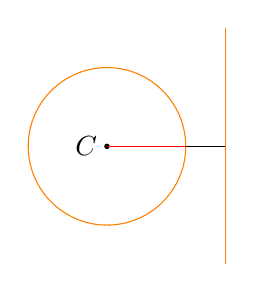
\begin{tikzpicture}
			\fill (0,0) circle [radius=1pt] node[left]{$C$};
			\draw[color=orange] (0,0) circle (1);
			\draw[color=orange] (1.5,1.5) -- (1.5,-1.5);
			\draw[color=black] (0,0)--(1.5,0);
			\draw[color=red] (0,0)--(1,0);
		\end{tikzpicture}
\end{minipage}
\begin{minipage}{0.7\textwidth}
		\begin{itemize}
			\item 相离
			\item $d>r$
			\item 没有交点
		\end{itemize}
\end{minipage}

\begin{minipage}{0.3\textwidth}
	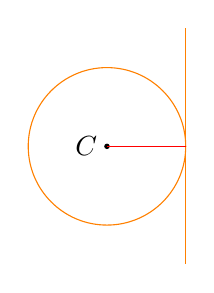
\begin{tikzpicture}
		\fill (0,0) circle [radius=1pt] node[left]{$C$};
		\draw[color=orange] (0,0) circle (1);
		\draw[color=orange] (1,1.5) -- (1,-1.5);
		\draw[color=black] (0,0)--(1,0);
		\draw[color=red] (0,0)--(1,0);
	\end{tikzpicture}
\end{minipage}
\begin{minipage}{0.7\textwidth}
	\begin{itemize}
		\item 相切
		\item $d=r$
		\item 有一个交点
	\end{itemize}
\end{minipage}

\begin{minipage}{0.3\textwidth}
	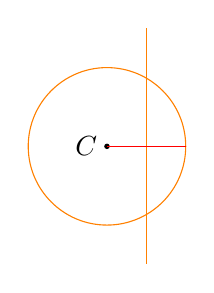
\begin{tikzpicture}
		\fill (0,0) circle [radius=1pt] node[left]{$C$};
		\draw[color=orange] (0,0) circle (1);
		\draw[color=orange] (0.5,1.5) -- (0.5,-1.5);
		\draw[color=black] (0,0)--(0.5,0);
		\draw[color=red] (0,0)--(1,0);
	\end{tikzpicture}
\end{minipage}
\begin{minipage}{0.7\textwidth}
	\begin{itemize}
		\item 相交
		\item $d<r$
		\item 有两个交点
	\end{itemize}
\end{minipage}

\section{直线与圆的位置关系 判定方法}

圆$ C: (x-a)^2+(y-b)^2=r^2(r>0) $

直线$ l: Ax+By+C=0 $ \vspace{20pt}

\subsection{几何法 判定}

借助圆心到直线的距离$d$与半径$r$的大小关系进行判定:\vspace{22pt}

\begin{minipage}{0.5\textwidth}
	\begin{itemize}
		\item $d>r$ $\Longleftrightarrow$ 相离
		\item $d=r$ $\Longleftrightarrow$ 相切
		\item $d<r$ $\Longleftrightarrow$ 相交
	\end{itemize}
\end{minipage}
\begin{minipage}{0.5\textwidth}
	提醒:\[ d= \frac{|Aa+Bb+C|}{\sqrt{A^2+B^2}} \]
\end{minipage}

\subsubsection{几何法 判定——例题}

			\textcolor[rgb]{0.15,0.7,0.15}{例1.} 判断直线$l$与圆$C$的位置关系:

			圆$C: x^2+y^2-2x-24=0$

			直线$l: x+y-2=0$. \vspace{40pt}

			\textcolor[rgb]{0.15,0.7,0.15}{练习1: }判断直线$l$与圆$C$的位置关系: 圆$C: x^2+y^2-2x-24=0$, \hspace{5pt}直线$l: 4x-3y+21=0$.

\subsection{代数法 判定}

借助直线与圆的公共点的个数进行判定:

\begin{displaymath}
\left\{ \begin{array}{l}
(x-a)^2+(y-b)^2=r^2 \\
Ax+By+C=0
\end{array} \right.
\Longrightarrow
\textbf{关于$x(y)$的一元二次方程}
\end{displaymath}

则其\textbf{解的个数}对应于\textbf{线圆交点个数}
\begin{itemize}
	\item $\Delta < 0$ $\Longleftrightarrow$ 没有交点 $\Longleftrightarrow$ 相离
	\item $\Delta = 0$ $\Longleftrightarrow$ 一个交点 $\Longleftrightarrow$ 相切
	\item $\Delta > 0$ $\Longleftrightarrow$ 两个交点 $\Longleftrightarrow$ 相交
\end{itemize}

\subsubsection{代数法 判定——例题}

			\textcolor[rgb]{0.15,0.7,0.15}{例2: }判断直线$l$与圆$C$的位置关系: 圆$C: x^2+y^2=4$, 直线$l: y=2x+1$. \vspace{22pt}

			\textcolor[rgb]{0.15,0.7,0.15}{练习2: }判断直线$l$与圆$C$的位置关系: 圆$C: x^2+y^2-2x-1=0$, \hspace{2pt}
			直线$l: x+y-2=0$.

\subsection{例题研究}

			\textcolor[rgb]{0.15,0.7,0.15}{例3: }若直线$ax+y=1$ 与圆$(x-1)^2+(y-2)^2=1$有两个不同的交点,求$a$的取值范围.\\\vspace{10pt}

			\textcolor[rgb]{0.15,0.7,0.15}{练习3: }直线 $y=kx+2$ 与圆 $x^2+y^2=1$ 没有公共点,则 $k$ 的取值范围是\underline{\hspace{25pt}}.

			\subsubsection{弦长问题}

			\textcolor[rgb]{0.15,0.7,0.15}{例4:}求直线$x-\sqrt{3}y+2\sqrt{3}=0$ 被圆$x^2+y^2=4$ 截得的弦长.
			\vspace{42pt}

			\textcolor[rgb]{0.15,0.7,0.15}{例5: } 直线过点$(4,0)$, 且被圆$x^2+y^2-2x-2y-7=0$所截得的弦长最长,求直线的方程为.\vspace{40pt}

\subsection{知识小结}
1. 直线与圆的位置关系判定:
\begin{description}
	\item[相离] $\Longleftrightarrow$ $d>r$ $\Longleftrightarrow$ $\Delta < 0$
	\item[相切] $\Longleftrightarrow$ $d=r$ $\Longleftrightarrow$ $\Delta = 0$
	\item[相交] $\Longleftrightarrow$ $d<r$ $\Longleftrightarrow$ $\Delta > 0$
\end{description}
% 圆心到直线的距离\[ d= \frac{|Aa+Bb+C|}{\sqrt{A^2+B^2}} \]

其中,\textbf{判别式$\Delta$}的来源:
\[\left\{ \begin{array}{l}
(x-a)^2+(y-b)^2=r^2 \\
Ax+By+C=0
\end{array} \right.
\Longrightarrow
\textbf{关于$x(y)$的一元二次方程}\]

2. 弦长问题:\vspace{22pt}

\begin{minipage}{0.5\textwidth}
	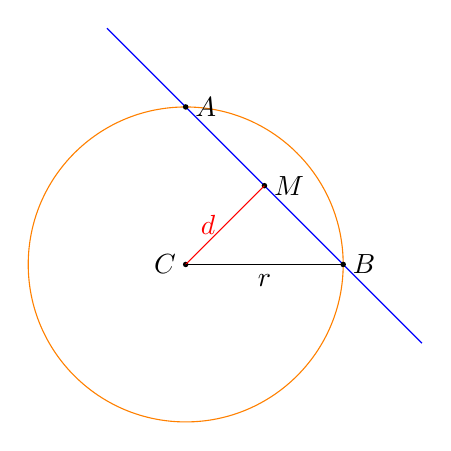
\begin{tikzpicture}
		\fill (0,0) circle [radius=1pt] node[left]{$C$};
		\draw[color=orange] (0,0) circle (2);
		\draw[color=blue] (-1,3) -- (3,-1);
		\fill (0,2) circle [radius=1pt] node[right]{$A$};
		\fill (2,0) circle [radius=1pt] node[right]{$B$};
		\fill (1,1) circle [radius=1pt] node[right]{$M$};
		\draw[color=red] (0,0)--(0.5,0.5)node[left]{$d$}--(1,1);
		\draw[color=black] (0,0)--(1,0)node[below]{$r$}--(2,0);
	\end{tikzpicture}
\end{minipage}
\begin{minipage}{0.5\textwidth}
	半径:$r$, 弦心距:$d$ \vspace{22pt}

	弦长:$ |AB|=2|BM|=2\sqrt{r^2-d^2} $
\end{minipage}


\vspace{22pt}
		\textbf{课后作业}

			《课时作业(二十八)》

\end{document}
